\chapter{Heaps and Heapsort}

So far you have met two sorting algorithms with very different personalities.
Insertion sort is simple and gentle and runs in $\Th(n^2)$ time in the worst
case. Merge sort is clever, divides and conquers, and runs in $\Th(n\log n)$
time --- but it pays for that speed with an extra array of scratch space the
size of the input. A natural question hangs in the air: \emph{can we sort in
$\Th(n\log n)$ time without borrowing a second array?}

The answer is yes, and the tool that gets us there is the \textbf{binary heap}.
A heap is a tree that lives inside a plain array, with no pointers, no
allocation, no fuss. Understanding it buys you two things at once. The first is
\textbf{heapsort}: an in-place, worst-case $\Th(n\log n)$ sorting algorithm. The
second is the \textbf{priority queue}: a tiny, fast scheduler that answers
the question ``what is the most important thing waiting right now?'' over and
over, and which we will lean on heavily later when we build Dijkstra's algorithm
and Prim's algorithm for graphs.

This chapter slows everything down. We will build the array-as-tree picture by
hand, trace every operation on real numbers, prove the loop invariants, and
derive --- not merely state --- the surprising fact that you can turn a random
array into a heap in \emph{linear} time.

\section{The shape of a heap}

\subsection{A tree hiding in an array}

Picture a binary tree. Not a search tree --- forget everything you might know
about ``smaller on the left, bigger on the right.'' Just a tree where every node
has at most two children. We are going to insist on one strict shape rule:

\begin{focusbox}
A \textbf{complete binary tree} is filled level by level, top to bottom, and
within each level left to right. Every level is completely full except possibly
the last, and the last level is packed as far to the left as it will go. There
are no gaps.
\end{focusbox}

That ``no gaps'' rule is what lets us drop the pointers. If the tree has no
holes, we can lay the nodes out in an array just by reading them off level by
level, and then a child's position is always a fixed arithmetic step away from
its parent's. Here is what that looks like.

\begin{center}
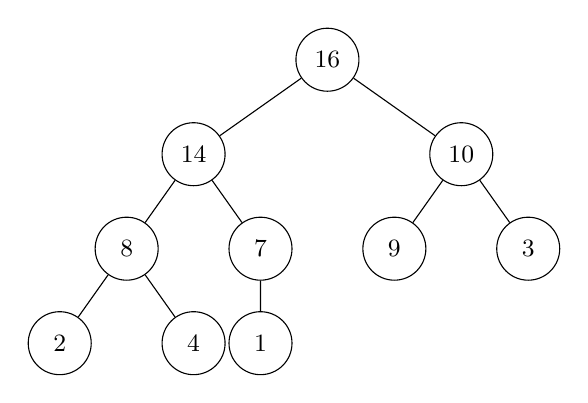
\begin{tikzpicture}[
  every node/.style={circle,draw,minimum size=8mm,inner sep=1pt,font=\small},
  level distance=12mm,
  level 1/.style={sibling distance=34mm},
  level 2/.style={sibling distance=17mm},
]
\node {16}
  child {node {14}
    child {node {8}
      child {node {2}}
      child {node {4}}
    }
    child {node {7}
      child {node {1}}
    }
  }
  child {node {10}
    child {node {9}}
    child {node {3}}
  };
\end{tikzpicture}
\end{center}

Now read those nodes off level by level: $16, 14, 10, 8, 7, 9, 3, 2, 4, 1$. Drop
them into an array, and (following CLRS) we will index that array starting from
$1$, not $0$, because the arithmetic comes out cleaner:

\begin{center}
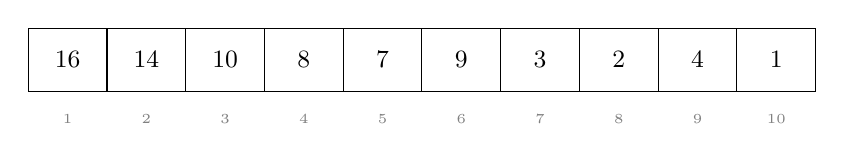
\begin{tikzpicture}[font=\small]
\foreach \val/\i [count=\j from 0] in {16/1,14/2,10/3,8/4,7/5,9/6,3/7,2/8,4/9,1/10} {
  \draw (\j,0) rectangle ++(1,0.8);
  \node at (\j+0.5,0.4) {\val};
  \node[gray] at (\j+0.5,-0.35) {\tiny \i};
}
\end{tikzpicture}
\end{center}

The gray numbers underneath are array indices. Stare at the tree and the array
together. The root $16$ is at index $1$. Its children, $14$ and $10$, are at
indices $2$ and $3$. The children of $14$ (index $2$) are $8$ and $7$, at indices
$4$ and $5$. The children of $10$ (index $3$) are $9$ and $3$, at indices $6$ and
$7$. A pattern is forming.

\begin{focusbox}
For a 1-indexed array, the node at index $i$ has
\[
  \mathrm{Parent}(i) = \floor{i/2}, \qquad
  \mathrm{Left}(i) = 2i, \qquad
  \mathrm{Right}(i) = 2i + 1.
\]
\end{focusbox}

Check it on index $2$: its left child is $2\cdot 2 = 4$ (the value $8$) and its
right child is $2\cdot 2 + 1 = 5$ (the value $7$). Its parent is
$\floor{2/2} = 1$ (the root). Every one of these is a single multiply, add, or
shift. On real hardware, doubling is a left bit-shift and halving is a right
bit-shift, so these are about the cheapest operations a computer can do.

\begin{intuitionbox}
A heap is a \emph{tree you can think about} but an \emph{array you can store}.
You get the conceptual clarity of a tree --- parents, children, levels, height
--- with the memory layout and cache-friendliness of a flat array. There are no
nodes to allocate and no pointers to chase or break. The tree structure is
entirely \emph{implied} by the index arithmetic.
\end{intuitionbox}

\begin{trapbox}
The most common beginner stumble: doing this with 0-indexed arrays but using the
1-indexed formulas. If your language indexes from $0$ (most do), the formulas
shift to $\mathrm{Left}(i) = 2i + 1$, $\mathrm{Right}(i) = 2i + 2$, and
$\mathrm{Parent}(i) = \floor{(i-1)/2}$. Pick a convention and \emph{write it at
the top of your code}. In this chapter we follow CLRS and index from $1$.
\end{trapbox}

\subsection{The heap property: the ordering rule}

The shape rule (complete tree) tells us \emph{where} things go. We now add an
\emph{ordering} rule that tells us how the values relate. There are two flavors.

\begin{formalbox}
An array $A[1\ldots n]$ is a \textbf{max-heap} if, for every node $i$ other than
the root,
\[
  A[\mathrm{Parent}(i)] \ge A[i].
\]
Equivalently: every parent is at least as large as each of its children. It is a
\textbf{min-heap} if instead $A[\mathrm{Parent}(i)] \le A[i]$ everywhere.
\end{formalbox}

Look back at our example tree. The root is $16$, the largest value. Below $16$
sit $14$ and $10$, both smaller. Below $14$ sit $8$ and $7$; below $10$ sit $9$
and $3$. Walk down any path from the root to a leaf and the values only ever
\emph{decrease} (or stay equal). That is a max-heap.

\begin{trapbox}
A heap is \textbf{not} a sorted array, and it is \textbf{not} a binary search
tree. In a max-heap the only promise is parent $\ge$ children. There is
\emph{no} relationship enforced between a node and its sibling, or between an
uncle and a niece, or between the two subtrees. In our example, $9$ (deep on the
right) is bigger than $8$, $7$, $2$, $4$, and $1$ (all on the left), even though
those left nodes sit higher in the tree. The heap property is purely local:
parent versus child, and nothing more. This local-ness is exactly what makes
heaps cheap to maintain.
\end{trapbox}

For the rest of the chapter we work with max-heaps; min-heaps are the mirror
image, obtained by flipping every $\ge$ to $\le$.

\begin{focusbox}
A heap actually has two pieces of bookkeeping. The array $A$ has some allocated
length, written $A.\mathit{length}$. But only the first $A.\mathit{heapsize}$
elements are ``in the heap'' right now, with $0 \le A.\mathit{heapsize} \le
A.\mathit{length}$. Elements past the heap size are still physically in the
array but are not part of the tree. This split will be the secret to making
heapsort in-place: as we extract elements, the heap shrinks and the sorted
region grows, all inside one array.
\end{focusbox}

\subsection{How tall is a heap?}

The height of a tree is the number of edges on the longest path from the root
down to a leaf. Because a heap is a complete binary tree, its height is tightly
controlled by the number of elements.

\begin{lemma}[Height of a heap]
\label{ch06:height}
A heap with $n$ elements has height $h = \floor{\log_2 n}$.
\end{lemma}

\begin{intuitionbox}
Each new level of a binary tree can hold twice as many nodes as the one above
it: level $0$ holds $1$ node, level $1$ holds up to $2$, level $2$ up to $4$, and
in general level $k$ holds up to $2^k$ nodes. To pile up $n$ nodes you need about
$\log_2 n$ levels, because doubling $\log_2 n$ times is what gets you to $n$. So
the tree is short and wide: $n = 1{,}000{,}000$ items fit in a tree only $20$
levels tall.
\end{intuitionbox}

\begin{formalbox}
A complete binary tree of height $h$ has at least $2^h$ nodes (the levels
$0$ through $h-1$ are completely full, contributing $1+2+\cdots+2^{h-1} =
2^h - 1$ nodes, plus at least one node on level $h$) and at most $2^{h+1}-1$
nodes (every level full). Hence
\[
  2^h \le n \le 2^{h+1}-1 < 2^{h+1}.
\]
Taking $\log_2$ of $2^h \le n < 2^{h+1}$ gives $h \le \log_2 n < h+1$, so
$h = \floor{\log_2 n} = \Th(\log n)$.
\end{formalbox}

This $\Th(\log n)$ height, recorded in Lemma~\ref{ch06:height}, is the source of
every speed claim in the chapter. The basic heap operations all do work
proportional to the height, so they all cost $\Oh(\log n)$.

\section{Max-heapify: repairing one broken spot}

Here is the workhorse. Suppose you have an array that is \emph{almost} a heap.
Specifically, you point at a node $i$, and you are promised that the left subtree
of $i$ and the right subtree of $i$ are both already valid max-heaps. The only
possible problem is at $i$ itself: maybe $A[i]$ is smaller than one of its
children, which would violate the heap property right there. The procedure
\textsc{Max-Heapify} fixes that single violation by letting the value at $i$
``sink'' or ``float down'' to where it belongs.

\begin{intuitionbox}
Think of a too-small value sitting at the top of two good heaps as a bubble of
air trapped under water. It does not belong up high. \textsc{Max-Heapify} lets it
sink, one level at a time, swapping past the larger of its two children, until
either it is bigger than both children or it has hit the bottom. As it sinks, the
bigger child rises to take the parent's place --- exactly what the heap property
wants up top.
\end{intuitionbox}

\begin{algorithm}[H]
\caption{\textsc{Max-Heapify}$(A, i)$ --- sink the value at $i$ into place}
\KwIn{Array $A$ with heap size $A.\mathit{heapsize}$; index $i$ whose two child subtrees are already max-heaps.}
\KwOut{The subtree rooted at $i$ is now a valid max-heap.}
$l \leftarrow \mathrm{Left}(i)$\;
$r \leftarrow \mathrm{Right}(i)$\;
\eIf{$l \le A.\mathit{heapsize}$ \textbf{and} $A[l] > A[i]$}{
  $\mathit{largest} \leftarrow l$\;
}{
  $\mathit{largest} \leftarrow i$\;
}
\If{$r \le A.\mathit{heapsize}$ \textbf{and} $A[r] > A[\mathit{largest}]$}{
  $\mathit{largest} \leftarrow r$\;
}
\If{$\mathit{largest} \ne i$}{
  exchange $A[i] \leftrightarrow A[\mathit{largest}]$\;
  \textsc{Max-Heapify}$(A, \mathit{largest})$\;
}
\end{algorithm}

Read it slowly. We find the index of the largest among the node and its two
children (carefully checking that each child actually exists, i.e.\ its index is
within the heap size). If the node itself is already the largest, there is
nothing to do --- the heap property holds here and we stop. Otherwise we swap the
node with its largest child, which fixes the violation at $i$, and then we
recurse on the child we swapped into, because the swap may have created a new
violation one level down.

\subsection{A full numeric trace}

Let us run \textsc{Max-Heapify}$(A, 2)$ on this array, where the subtrees are
valid heaps but the value at index $2$ is too small. Take
\[
  A = [\,16,\ \mathbf{4},\ 10,\ 14,\ 7,\ 9,\ 3,\ 2,\ 8,\ 1\,],
  \qquad \mathit{heapsize} = 10.
\]
As a tree, with the offending $4$ in red:

\begin{center}
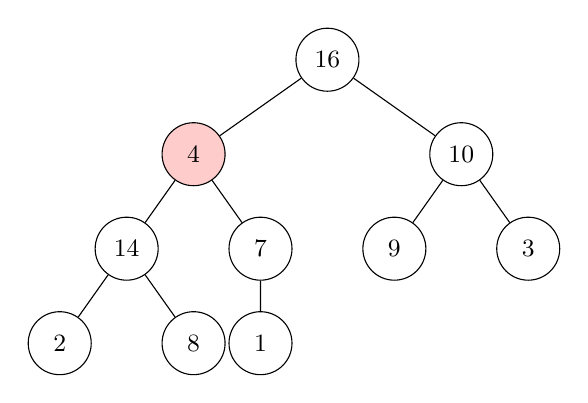
\begin{tikzpicture}[
  every node/.style={circle,draw,minimum size=8mm,inner sep=1pt,font=\small},
  level distance=12mm,
  level 1/.style={sibling distance=34mm},
  level 2/.style={sibling distance=17mm},
]
\node {16}
  child {node[fill=red!20] {4}
    child {node {14}
      child {node {2}}
      child {node {8}}
    }
    child {node {7}
      child {node {1}}
    }
  }
  child {node {10}
    child {node {9}}
    child {node {3}}
  };
\end{tikzpicture}
\end{center}

\textbf{Call \textsc{Max-Heapify}$(A,2)$.} Here $i=2$, so $l=4$ and $r=5$. The
values are $A[2]=4$, $A[4]=14$, $A[5]=7$. The largest of $\{4,14,7\}$ is $14$ at
index $4$, so $\mathit{largest}=4 \ne i$. We swap $A[2] \leftrightarrow A[4]$:
\[
  A = [\,16,\ 14,\ 10,\ \mathbf{4},\ 7,\ 9,\ 3,\ 2,\ 8,\ 1\,].
\]
The $14$ has floated up; the $4$ has dropped to index $4$. Now we recurse on
index $4$.

\textbf{Call \textsc{Max-Heapify}$(A,4)$.} Now $i=4$, so $l=8$ and $r=9$. Values:
$A[4]=4$, $A[8]=2$, $A[9]=8$. The largest of $\{4,2,8\}$ is $8$ at index $9$, so
$\mathit{largest}=9$. Swap $A[4] \leftrightarrow A[9]$:
\[
  A = [\,16,\ 14,\ 10,\ 8,\ 7,\ 9,\ 3,\ 2,\ \mathbf{4},\ 1\,].
\]
Recurse on index $9$.

\textbf{Call \textsc{Max-Heapify}$(A,9)$.} Now $i=9$, so $l=18$ and $r=19$. Both
exceed $\mathit{heapsize}=10$, so node $9$ has no children --- it is a leaf.
Thus $\mathit{largest}=i$, the test $\mathit{largest}\ne i$ fails, and we stop.

The $4$ has sunk all the way to a leaf, and the array is now a valid max-heap:

\begin{center}
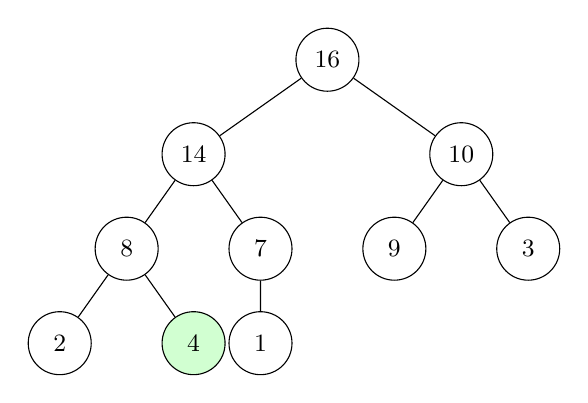
\begin{tikzpicture}[
  every node/.style={circle,draw,minimum size=8mm,inner sep=1pt,font=\small},
  level distance=12mm,
  level 1/.style={sibling distance=34mm},
  level 2/.style={sibling distance=17mm},
]
\node {16}
  child {node {14}
    child {node {8}
      child {node {2}}
      child {node[fill=green!18] {4}}
    }
    child {node {7}
      child {node {1}}
    }
  }
  child {node {10}
    child {node {9}}
    child {node {3}}
  };
\end{tikzpicture}
\end{center}

Notice the path the $4$ took: index $2 \to 4 \to 9$, exactly one node per level,
straight down the tree. That is the crucial observation for the running time.

\subsection{Why it is correct}

\begin{focusbox}
\textbf{The promise \textsc{Max-Heapify} relies on.} It is only correct if, when
you call it on $i$, the subtrees rooted at $\mathrm{Left}(i)$ and
$\mathrm{Right}(i)$ are \emph{already} valid max-heaps. The procedure fixes a
violation \emph{at} $i$; it cannot fix a mess scattered throughout the subtrees.
\end{focusbox}

Given that promise, here is the gentle correctness argument, by induction on the
height of node $i$.

\begin{itemize}
\item \textbf{Base case.} If $i$ is a leaf, it has no children, so
$\mathit{largest}=i$ and the procedure does nothing. A single node is trivially a
max-heap. Correct.
\item \textbf{Inductive step.} Suppose \textsc{Max-Heapify} is correct on every
node of height less than $h$, and let $i$ have height $h$. We pick
$\mathit{largest}$ to be the index of the maximum of $A[i]$, $A[l]$, $A[r]$. If
$\mathit{largest}=i$, then $A[i]$ already dominates both children; combined with
the promise that the subtrees are heaps, the whole subtree at $i$ is a heap, and
we correctly stop. If instead $\mathit{largest}\ne i$, we swap, which places the
true maximum at $i$ --- so the heap property now holds between $i$ and both of
its children. The swap may have lowered a value into the child at
$\mathit{largest}$, possibly breaking the property there; but the two subtrees of
$\mathit{largest}$ were untouched and are still heaps, so the promise holds for
the recursive call. That child has height $h-1 < h$, so by the inductive
hypothesis the recursive call repairs it. The subtree at $i$ is now fully a
max-heap.
\end{itemize}

\subsection{Cost of \textsc{Max-Heapify}}

Each call does a constant amount of work --- a few comparisons and at most one
swap --- and then either stops or recurses on a node one level down. So the total
work is proportional to the number of levels the value sinks, which is at most
the height $h$ of the starting node. Since the height of any node is at most
$\floor{\log_2 n}$ (Lemma~\ref{ch06:height}), we get the following.

\begin{complexitybox}
\textsc{Max-Heapify} on a node of height $h$ runs in $\Oh(h)$ time, hence
$\Oh(\log n)$ in the worst case on an $n$-element heap. It uses $\Oh(1)$ extra
space if written as a loop (the recursion is tail recursion and turns into a
\textbf{while} loop with no stack growth).
\end{complexitybox}

\begin{remark}
You can also bound the recurrence directly. A subtree of $n$ nodes has children
subtrees of at most $2n/3$ nodes each (the worst case is when the bottom level is
exactly half full). So the running time obeys $T(n) \le T(2n/3) + \Th(1)$, which
by the master theorem (case 2 with $a=1$, $b=3/2$) solves to $T(n) = \Oh(\log
n)$. Same answer, arrived at two ways.
\end{remark}

\begin{walkbox}
Convince yourself that \textsc{Max-Heapify} really only walks one root-to-leaf
path and never branches sideways. Why can it never need to ``go back up''? Think
about what is true above $i$ before the call and whether any swap can disturb it.
\end{walkbox}

\section{Build-Max-Heap: a heap from chaos}

We can fix one broken spot. How do we turn a completely arbitrary array into a
heap? The clean idea: call \textsc{Max-Heapify} on every node, but in the
\emph{right order}. \textsc{Max-Heapify} demands that a node's subtrees already
be heaps, so we must process nodes \textbf{bottom-up} --- repair the small
subtrees first, then larger ones built on top of them.

\begin{focusbox}
Here is a free fact that cuts our work in half. In an array of size $n$, the
elements indexed $\floor{n/2}+1, \floor{n/2}+2, \ldots, n$ are exactly the
\emph{leaves} of the tree. A leaf has no children, so it is already a
one-element max-heap --- nothing to fix. We only need to run
\textsc{Max-Heapify} on the internal nodes, indices $1$ through $\floor{n/2}$,
and we sweep them in \emph{decreasing} order so children are handled before
parents.
\end{focusbox}

\begin{algorithm}[H]
\caption{\textsc{Build-Max-Heap}$(A)$ --- heapify an arbitrary array}
\KwIn{Array $A[1\ldots n]$ in any order.}
\KwOut{$A$ rearranged in place into a max-heap.}
$A.\mathit{heapsize} \leftarrow A.\mathit{length}$\;
\For{$i \leftarrow \floor{A.\mathit{length}/2}$ \textbf{downto} $1$}{
  \textsc{Max-Heapify}$(A, i)$\;
}
\end{algorithm}

\subsection{A full numeric trace}

Take the unordered array
\[
  A = [\,4,\ 1,\ 3,\ 2,\ 16,\ 9,\ 10,\ 14,\ 8,\ 7\,], \qquad n = 10.
\]
The internal nodes are indices $1$ through $\floor{10/2}=5$. We process
$i = 5, 4, 3, 2, 1$.

\textbf{$i=5$:} node $A[5]=16$, children $A[10]=7$ only ($A[11]$ doesn't exist).
$16 > 7$, no swap needed.

\textbf{$i=4$:} node $A[4]=2$, children $A[8]=14$, $A[9]=8$. Largest is $14$;
swap. Now $A[4]=14$, $A[8]=2$. The new node $A[8]=2$ is a leaf; stop.
\[
  A = [\,4,\ 1,\ 3,\ 14,\ 16,\ 9,\ 10,\ 2,\ 8,\ 7\,].
\]

\textbf{$i=3$:} node $A[3]=3$, children $A[6]=9$, $A[7]=10$. Largest is $10$;
swap. $A[3]=10$, $A[7]=3$. Node $A[7]=3$ is a leaf; stop.
\[
  A = [\,4,\ 1,\ 10,\ 14,\ 16,\ 9,\ 3,\ 2,\ 8,\ 7\,].
\]

\textbf{$i=2$:} node $A[2]=1$, children $A[4]=14$, $A[5]=16$. Largest is $16$;
swap. $A[2]=16$, $A[5]=1$. Recurse on index $5$: $A[5]=1$, child $A[10]=7$;
largest is $7$, swap, $A[5]=7$, $A[10]=1$. Node $10$ is a leaf; stop.
\[
  A = [\,4,\ 16,\ 10,\ 14,\ 7,\ 9,\ 3,\ 2,\ 8,\ 1\,].
\]

\textbf{$i=1$:} node $A[1]=4$, children $A[2]=16$, $A[3]=10$. Largest is $16$;
swap. $A[1]=16$, $A[2]=4$. Recurse on index $2$: this is exactly the
\textsc{Max-Heapify}$(A,2)$ we traced earlier! The $4$ sinks $2\to 4\to 9$,
giving
\[
  A = [\,16,\ 14,\ 10,\ 8,\ 7,\ 9,\ 3,\ 2,\ 4,\ 1\,].
\]

That is a valid max-heap --- the very tree we drew at the start of the chapter.

\subsection{Why it is correct: a loop invariant}

\begin{formalbox}
\textbf{Loop invariant for \textsc{Build-Max-Heap}.} At the start of each
iteration of the \textbf{for} loop with counter $i$, each of the nodes
$i+1, i+2, \ldots, n$ is the root of a valid max-heap.
\end{formalbox}

\textbf{Initialization.} Before the first iteration, $i = \floor{n/2}$, so the
nodes $i+1,\ldots,n$ are exactly the leaves. Every leaf is a one-node heap, so
the invariant holds.

\textbf{Maintenance.} Consider an iteration with counter $i$. The children of $i$
are indexed $2i$ and $2i+1$, both \emph{strictly greater} than $i$, so by the
invariant they are already roots of valid max-heaps. That is exactly the promise
\textsc{Max-Heapify}$(A,i)$ requires, so after it runs, node $i$ is the root of a
max-heap too. The higher-indexed nodes were not touched, so they remain heaps.
Decrementing $i$ reestablishes the invariant for the next iteration.

\textbf{Termination.} The loop ends when $i=0$. The invariant then says nodes
$1,\ldots,n$ are all roots of max-heaps. In particular node $1$, the root of the
whole tree, is a max-heap --- which is exactly what we wanted.

\subsection{The surprising linear-time analysis}

Here is the part people get wrong. The lazy estimate says: we call
\textsc{Max-Heapify} on $\Oh(n)$ nodes, and each call costs $\Oh(\log n)$, so the
total is $\Oh(n\log n)$. That bound is \emph{correct but loose}. The truth is
better: \textsc{Build-Max-Heap} runs in $\Oh(n)$ time. Let us see why.

\begin{intuitionbox}
The $\Oh(n\log n)$ estimate pretends every node sinks all the way down through
$\log n$ levels. But most nodes are near the bottom and barely sink at all! Half
the nodes are leaves (sink $0$), a quarter are one level up (sink at most $1$), an
eighth sink at most $2$, and so on. The cheap, numerous nodes vastly outnumber
the expensive, rare ones near the root. Add up the real costs and the total
collapses to linear.
\end{intuitionbox}

The picture below makes the imbalance visible. Each row is a level of the tree;
the rows near the bottom are crowded with cheap nodes, while the expensive nodes
near the top are few. The arrow on the right of each row is the most a node on
that row can sink.

\begin{center}
\begin{tikzpicture}[font=\small,node distance=0pt]
% rows drawn top-to-bottom; \row is the drawing row (0 at top),
% \hgt is the height of nodes on that row, \cnt the count, \sink the max sink.
\foreach \row/\hgt/\cnt/\sink in {0/3/1/3, 1/2/1/2, 2/1/3/1, 3/0/5/0} {
  \pgfmathsetmacro{\y}{-\row*0.85}
  \pgfmathsetmacro{\start}{-\cnt*0.5}
  \foreach \k in {1,...,\cnt} {
    \pgfmathsetmacro{\x}{\start + (\k-1)*1.0 + 0.5}
    \node[circle,draw,minimum size=6mm,inner sep=0pt,
      fill={\ifnum\hgt>1 structurepurple!18\else targetgreen!18\fi}] at (\x,\y) {};
  }
  \node[anchor=west] at (3.2,\y)
    {height \hgt: $\sim n/2^{\hgt+1}$ nodes, each sinks $\le \sink$};
}
\end{tikzpicture}
\end{center}

This is a $10$-node heap, so the counts are small; in a large heap the doubling
is exact and each row down holds twice as many nodes as the one above. Notice how
the green bottom rows --- the cheap, numerous nodes near height $0$ --- dwarf the
purple top rows near the root. That visual imbalance is the whole secret.

Let us count carefully. A \textsc{Max-Heapify} call on a node of height $h$ costs
$\Oh(h)$. So we need to know: how many nodes have each height? In a heap with $n$
elements, the number of nodes at height $h$ is at most $\ceil{n/2^{h+1}}$.

\begin{focusbox}
Why $\ceil{n/2^{h+1}}$? Height-$0$ nodes are the leaves: there are about $n/2$ of
them ($\ceil{n/2}$ exactly). Height-$1$ nodes are about $n/4$, height-$2$ are
about $n/8$. Each step up the tree halves the count, so height-$h$ nodes number
about $n/2^{h+1}$.
\end{focusbox}

The total cost of \textsc{Build-Max-Heap} is therefore at most
\[
  \sum_{h=0}^{\floor{\log_2 n}} \ceil{\frac{n}{2^{h+1}}}\, \Oh(h)
  \;=\; \Oh\!\left( n \sum_{h=0}^{\floor{\log_2 n}} \frac{h}{2^{h+1}} \right)
  \;=\; \Oh\!\left( n \sum_{h=0}^{\infty} \frac{h}{2^{h}} \right).
\]
Everything now hinges on that last infinite sum, $\sum_{h=0}^{\infty} h/2^{h}$.
This is a standard series. Using the identity $\sum_{h=0}^{\infty} h x^{h} =
x/(1-x)^2$ for $\abs{x}<1$, plug in $x = 1/2$:
\[
  \sum_{h=0}^{\infty} \frac{h}{2^{h}}
  = \frac{1/2}{(1 - 1/2)^2}
  = \frac{1/2}{1/4}
  = 2.
\]
The sum is a \emph{constant}, namely $2$. Therefore
\[
  \text{cost of \textsc{Build-Max-Heap}} = \Oh\!\left(n \cdot 2\right) = \Oh(n).
\]

\begin{complexitybox}
\textsc{Build-Max-Heap} converts an arbitrary $n$-element array into a max-heap
in $\Th(n)$ time --- \textbf{linear}, not $n\log n$. It works in place, using
$\Oh(1)$ extra space.
\end{complexitybox}

\begin{intuitionbox}
The intuition behind ``the sum is just $2$'': the nodes that are expensive to
sink (high up, large $h$) are exponentially rare, while the cheap nodes (low
down, small $h$) are exponentially common. The geometric decay of the counts
overwhelms the linear growth of the per-node cost. This tension between a
linearly growing weight and a geometrically shrinking population, resolving to a
constant, is a pattern you will meet again and again in algorithm analysis.
\end{intuitionbox}

\begin{trapbox}
If you build a heap by \emph{inserting} elements one at a time instead (a method
we will meet under priority queues), each insertion costs $\Oh(\log n)$ and the
total really is $\Th(n\log n)$ in the worst case. The clever bottom-up
\textsc{Build-Max-Heap} is faster precisely because it does most of its work near
the cheap bottom of the tree. Do not confuse the two construction methods.
\end{trapbox}

\section{Heapsort}

Now the payoff. We have a max-heap, so the largest element of the whole array is
sitting right at the root, index $1$. Notice where that wants to end up: in a
sorted array (ascending), the largest element belongs at the \emph{end}. So:

\begin{intuitionbox}
\textbf{The heapsort move.} The maximum is at the front (index $1$). The slot it
ultimately belongs in is the back. So swap them: put the max where it belongs at
the end, and bring the back element up to the root. Now shrink the heap by one so
that the parked maximum is ``out of the game,'' and call \textsc{Max-Heapify} on
the root to fix the one violation we just created. The new maximum bubbles up to
the root, and we repeat. Each round freezes one more element into its correct
final place at the growing sorted tail.
\end{intuitionbox}

The single move is worth a picture. The largest element lives at the front of the
heap; the sorted tail grows at the back. One step swaps them, shrinks the heap
boundary leftward by one, and re-heapifies the front:

\begin{center}
\begin{tikzpicture}[font=\small]
% top row: before
\foreach \val/\i [count=\j from 0] in {16/1,14/2,10/3,8/4,7/5,9/6,3/7,2/8,4/9,1/10} {
  \draw[fill={\ifnum\i=1 sourceblue!22\else\ifnum\i=10 quotientorange!22\else white\fi\fi}]
    (\j,1.2) rectangle ++(0.85,0.7);
  \node at (\j+0.425,1.55) {\val};
}
\draw[->,thick,sourceblue] (0.425,2.05) to[bend left=40] node[above,font=\scriptsize]{swap} (9.0,2.05);
% bottom row: after swap+shrink (heapified)
\foreach \val/\i [count=\j from 0] in {14/1,8/2,10/3,4/4,7/5,9/6,3/7,2/8,1/9,16/10} {
  \draw[fill={\ifnum\i=10 quotientorange!22\else white\fi}]
    (\j,0) rectangle ++(0.85,0.7);
  \node at (\j+0.425,0.35) {\val};
}
% heap-boundary bar after shrink (between index 9 and 10)
\draw[very thick,trapred] (9.0,-0.15) -- (9.0,0.85);
\node[trapred,font=\scriptsize,anchor=north] at (9.0,-0.15) {frozen};
\node[font=\scriptsize,anchor=east] at (-0.15,1.55) {heap};
\node[font=\scriptsize,anchor=east] at (-0.15,0.35) {after};
\end{tikzpicture}
\end{center}

The blue root and the orange last slot trade places; the red bar then walls off
the now-frozen maximum, and \textsc{Max-Heapify} repairs the shrunken heap on its
left.

\begin{algorithm}[H]
\caption{\textsc{Heapsort}$(A)$ --- sort an array ascending, in place}
\KwIn{Array $A[1\ldots n]$ in any order.}
\KwOut{$A$ sorted in nondecreasing order.}
\textsc{Build-Max-Heap}$(A)$\;
\For{$i \leftarrow A.\mathit{length}$ \textbf{downto} $2$}{
  exchange $A[1] \leftrightarrow A[i]$\;
  $A.\mathit{heapsize} \leftarrow A.\mathit{heapsize} - 1$\;
  \textsc{Max-Heapify}$(A, 1)$\;
}
\end{algorithm}

\subsection{Watching it run}

Start from the heap we built, $A = [16,14,10,8,7,9,3,2,4,1]$, heap size $10$. We
will track the array; a vertical bar $\mid$ marks the boundary between the
shrinking heap (left) and the sorted tail (right).

\begin{center}
\renewcommand{\arraystretch}{1.25}
\begin{tabular}{r l}
\toprule
step & array \\
\midrule
start         & $16\ 14\ 10\ 8\ 7\ 9\ 3\ 2\ 4\ 1$ \\
swap $1\leftrightarrow10$, shrink, heapify
              & $14\ 8\ 10\ 4\ 7\ 9\ 3\ 2\ 1 \mid 16$ \\
swap $1\leftrightarrow 9$, shrink, heapify
              & $10\ 8\ 9\ 4\ 7\ 1\ 3\ 2 \mid 14\ 16$ \\
swap $1\leftrightarrow 8$, shrink, heapify
              & $9\ 8\ 3\ 4\ 7\ 1\ 2 \mid 10\ 14\ 16$ \\
swap $1\leftrightarrow 7$, shrink, heapify
              & $8\ 7\ 3\ 4\ 2\ 1 \mid 9\ 10\ 14\ 16$ \\
swap $1\leftrightarrow 6$, shrink, heapify
              & $7\ 4\ 3\ 1\ 2 \mid 8\ 9\ 10\ 14\ 16$ \\
swap $1\leftrightarrow 5$, shrink, heapify
              & $4\ 2\ 3\ 1 \mid 7\ 8\ 9\ 10\ 14\ 16$ \\
swap $1\leftrightarrow 4$, shrink, heapify
              & $3\ 2\ 1 \mid 4\ 7\ 8\ 9\ 10\ 14\ 16$ \\
swap $1\leftrightarrow 3$, shrink, heapify
              & $2\ 1 \mid 3\ 4\ 7\ 8\ 9\ 10\ 14\ 16$ \\
swap $1\leftrightarrow 2$, shrink, heapify
              & $1 \mid 2\ 3\ 4\ 7\ 8\ 9\ 10\ 14\ 16$ \\
\midrule
done          & $1\ 2\ 3\ 4\ 7\ 8\ 9\ 10\ 14\ 16$ \\
\bottomrule
\end{tabular}
\end{center}

Watch the sorted tail on the right grow leftward, one frozen element per step,
always pulling the current maximum out of the heap and dropping it just to the
left of the previously frozen values. When the heap is down to a single element,
that element is automatically the smallest, already in place, and we are done.

\begin{labbox}
\textbf{Trace it yourself.} Take $A = [5, 13, 2, 25, 7, 17, 20, 8, 4]$ (nine
elements). First run \textsc{Build-Max-Heap} by hand: process indices $4,3,2,1$
in order, drawing the tree after each \textsc{Max-Heapify}. You should get a heap
with $25$ at the root. Then run the heapsort loop and confirm the array marches
to $[2,4,5,7,8,13,17,20,25]$. Check your work by verifying after every
\textsc{Max-Heapify} that no parent is smaller than a child --- if you ever spot
one, you slipped.
\end{labbox}

\subsection{Correctness via a loop invariant}

\begin{formalbox}
\textbf{Loop invariant for the heapsort loop.} At the start of each iteration
with counter $i$:
\begin{enumerate}
\item the subarray $A[i+1 \ldots n]$ is sorted and contains the $n-i$ largest
elements of the whole array, each in its final position; and
\item the subarray $A[1 \ldots i]$ is a valid max-heap on the current heap size
$i$.
\end{enumerate}
\end{formalbox}

\textbf{Initialization.} Before the first iteration $i=n$, so the sorted tail
$A[n+1\ldots n]$ is empty (vacuously sorted), and $A[1\ldots n]$ is a max-heap
because \textsc{Build-Max-Heap} just made it one.

\textbf{Maintenance.} In the iteration we swap $A[1]$ (the maximum of the current
heap) with $A[i]$. Because the heap held the $i$ largest unsorted elements and
$A[1]$ was their maximum, $A[1]$ is the largest element not yet placed --- so
moving it to position $i$, just before the sorted tail, keeps $A[i\ldots n]$
sorted and correct. Shrinking the heap to size $i-1$ removes that frozen element
from play. The swap put a possibly-small value at the root, breaking the heap
property only at index $1$; the two subtrees are untouched and still heaps, so
\textsc{Max-Heapify}$(A,1)$ restores a valid max-heap on $A[1\ldots i-1]$.
Decrementing $i$ reestablishes the invariant.

\textbf{Termination.} The loop ends at $i=1$. Then $A[2\ldots n]$ is sorted and
holds the $n-1$ largest elements, while $A[1]$ is the single remaining smallest
element. So the whole array $A[1\ldots n]$ is sorted. Done.

\subsection{Cost of heapsort}

\begin{complexitybox}
\textsc{Heapsort} runs in $\Th(n\log n)$ time in the worst case and uses
$\Oh(1)$ extra space (it sorts in place). The build phase is $\Th(n)$; the
extract phase does $n-1$ calls to \textsc{Max-Heapify}, each $\Oh(\log n)$, for
$\Oh(n\log n)$. The $\Th(n\log n)$ term dominates the $\Th(n)$ build.
\end{complexitybox}

The $\Om(n\log n)$ lower bound (so the running time is $\Th$, not merely $\Oh$)
comes from the fact that many inputs force the maximum element, after each
extraction, to sink a full $\Th(\log n)$ levels back down. We will not belabor
it, but the upper and lower bounds meet at $\Th(n\log n)$.

\begin{aestheticbox}
Heapsort is the algorithm you reach for when memory is precious and you must
guarantee $n\log n$ behavior on \emph{every} input. Quicksort (next chapter) is
usually faster in practice on real machines because of better cache behavior, but
it can degrade to $\Th(n^2)$ on adversarial inputs. Merge sort guarantees
$\Th(n\log n)$ but needs $\Th(n)$ scratch space. Heapsort threads the needle:
worst-case $\Th(n\log n)$ \emph{and} in-place. That is why it shows up in places
like the Linux kernel and in introsort (the hybrid behind many standard-library
sorts), which starts with quicksort and falls back to heapsort if recursion goes
too deep --- using heapsort precisely as the worst-case safety net.
\end{aestheticbox}

\begin{trapbox}
Heapsort is \textbf{not stable}: equal keys can be reordered relative to their
original positions, because the swaps fling elements across the array. If you
need stability (e.g.\ sorting records by one field while preserving an earlier
ordering on another), heapsort alone will not give it to you without extra
tie-breaking keys.
\end{trapbox}

\section{Priority queues}

The heap's second life is as a \textbf{priority queue}, and this is where
heaps earn their keep in real systems even more than in sorting. A priority queue
maintains a set $S$ of elements, each with an associated \emph{key} (its
priority), and supports operations that always let you get at the most important
element fast.

\begin{focusbox}
A max-priority-queue supports:
\begin{itemize}
\item \textsc{Insert}$(S, x)$ --- add element $x$ to the set.
\item \textsc{Maximum}$(S)$ --- return the element with the largest key.
\item \textsc{Extract-Max}$(S)$ --- remove and return the element with the
largest key.
\item \textsc{Increase-Key}$(S, x, k)$ --- raise element $x$'s key to the new,
larger value $k$.
\end{itemize}
A min-priority-queue is the mirror image (\textsc{Minimum},
\textsc{Extract-Min}, \textsc{Decrease-Key}) and is what shortest-path and
minimum-spanning-tree algorithms actually use.
\end{focusbox}

\begin{aestheticbox}
Priority queues are everywhere a system must repeatedly ask ``what next?'' An
operating-system scheduler picks the highest-priority runnable process. A
network router forwards the highest-priority packet. Event-driven simulations pull
the next event by time. Dijkstra's shortest-path algorithm repeatedly extracts
the closest unfinished vertex. Huffman coding repeatedly extracts the two
lowest-frequency symbols. In every case the heap gives you \textsc{Extract} and
\textsc{Insert} in $\Oh(\log n)$, which is what makes those algorithms efficient.
\end{aestheticbox}

\subsection{Maximum and Extract-Max}

Reading the maximum is trivial: it is the root.

\begin{algorithm}[H]
\caption{\textsc{Heap-Maximum}$(A)$}
\KwIn{Nonempty max-heap $A$.}
\KwOut{The maximum element.}
\Return $A[1]$\;
\end{algorithm}

Removing it reuses the heapsort move: take the root, plug the last leaf into the
root's slot, shrink, and heapify.

\begin{algorithm}[H]
\caption{\textsc{Heap-Extract-Max}$(A)$}
\KwIn{Max-heap $A$ with $A.\mathit{heapsize} \ge 1$.}
\KwOut{The maximum element, removed from the heap.}
\If{$A.\mathit{heapsize} < 1$}{\textbf{error} ``heap underflow''\;}
$\mathit{max} \leftarrow A[1]$\;
$A[1] \leftarrow A[A.\mathit{heapsize}]$\;
$A.\mathit{heapsize} \leftarrow A.\mathit{heapsize} - 1$\;
\textsc{Max-Heapify}$(A, 1)$\;
\Return $\mathit{max}$\;
\end{algorithm}

We save the root to return it, move the last element of the heap up to the root,
shrink the heap, and let \textsc{Max-Heapify} sink that moved element to its
proper place. One root-to-leaf path of work: $\Oh(\log n)$.

\textbf{Quick trace.} On $A=[16,14,10,8,7,9,3,2,4,1]$, \textsc{Heap-Extract-Max}
saves $16$, moves the last element $1$ into the root, shrinks to size $9$, giving
$[1,14,10,8,7,9,3,2,4]$, then heapifies the root: $1$ sinks $1\to 2\to 4\to 9$,
landing among the leaves, and the array becomes the valid heap
$[14,8,10,4,7,9,3,2,1]$ with $16$ returned. Compare this to the first heapsort
step --- it is the same operation.

\subsection{Increase-Key and Insert}

The remaining operations move a value \emph{up} the tree instead of down. If you
raise a node's key, it may now exceed its parent, so it should ``float up''
toward the root --- the opposite of sinking.

\begin{algorithm}[H]
\caption{\textsc{Heap-Increase-Key}$(A, i, \mathit{key})$ --- raise $A[i]$ and float it up}
\KwIn{Max-heap $A$, index $i$, and a new $\mathit{key} \ge A[i]$.}
\KwOut{Heap property restored after raising $A[i]$ to $\mathit{key}$.}
\If{$\mathit{key} < A[i]$}{\textbf{error} ``new key smaller than current key''\;}
$A[i] \leftarrow \mathit{key}$\;
\While{$i > 1$ \textbf{and} $A[\mathrm{Parent}(i)] < A[i]$}{
  exchange $A[i] \leftrightarrow A[\mathrm{Parent}(i)]$\;
  $i \leftarrow \mathrm{Parent}(i)$\;
}
\end{algorithm}

The \textbf{while} loop is the floating-up: as long as the node has a parent and
is bigger than that parent, swap them and climb. It is the structural twin of
\textsc{Max-Heapify}, walking a leaf-to-root path instead of a root-to-leaf one.

\textbf{Trace.} In $A=[16,14,10,8,7,9,3,2,4,1]$, call
\textsc{Heap-Increase-Key}$(A, 9, 15)$ --- raise the value at index $9$ (it is
$4$) up to $15$. Set $A[9]=15$. Its parent is index $\floor{9/2}=4$, value $8$.
Since $15 > 8$, swap: now $15$ is at index $4$, $8$ at index $9$. The parent of
index $4$ is index $2$, value $14$. Since $15 > 14$, swap: $15$ at index $2$,
$14$ at index $4$. The parent of index $2$ is index $1$, value $16$. Since
$15 < 16$, stop. The $15$ has floated up two levels to index $2$, and the heap is
valid again:
\[
  A = [\,16,\ 15,\ 10,\ 14,\ 7,\ 9,\ 3,\ 2,\ 8,\ 1\,].
\]

The path the raised key climbs is shown below: from index $9$ up through index
$4$ to its resting place at index $2$, stopping only when it meets a parent
($16$) at least as large.

\begin{center}
\begin{tikzpicture}[
  every node/.style={circle,draw,minimum size=8mm,inner sep=1pt,font=\small},
  level distance=12mm,
  level 1/.style={sibling distance=34mm},
  level 2/.style={sibling distance=17mm},
]
\node {16}
  child {node[fill=targetgreen!20] {15}
    child {node {14}
      child {node {2}}
      child {node[fill=structurepurple!18] {8}}
    }
    child {node {7}
      child {node {1}}
    }
  }
  child {node {10}
    child {node {9}}
    child {node {3}}
  };
\end{tikzpicture}
\end{center}

The green node is the raised key $15$ in its final spot; the purple node holds the
$8$ that the climb pushed down into the vacated slot at index $9$. Float-up is the
exact mirror of the sink in \textsc{Max-Heapify}: one node per level, along a
single path, comparing against just one neighbor (here the parent).

Insertion is then a small trick: append a sentinel of $-\infty$ as a new leaf
(growing the heap), then immediately \textsc{Increase-Key} it up to the real
value, which floats it to the correct spot.

\begin{algorithm}[H]
\caption{\textsc{Max-Heap-Insert}$(A, \mathit{key})$}
\KwIn{Max-heap $A$ and a $\mathit{key}$ to insert.}
\KwOut{$A$ with $\mathit{key}$ added, heap property intact.}
$A.\mathit{heapsize} \leftarrow A.\mathit{heapsize} + 1$\;
$A[A.\mathit{heapsize}] \leftarrow -\infty$\;
\textsc{Heap-Increase-Key}$(A, A.\mathit{heapsize}, \mathit{key})$\;
\end{algorithm}

\begin{intuitionbox}
\textsc{Max-Heapify} sinks values \emph{down} (used by extract and build);
\textsc{Heap-Increase-Key} floats values \emph{up} (used by insert and key
raises). Down-heap walks parent-to-children comparing against the larger child;
up-heap walks child-to-parent comparing against the one parent. Two directions,
one idea: restore a single local violation by walking the unique path along which
it could propagate.
\end{intuitionbox}

\begin{complexitybox}
On an $n$-element heap, all priority-queue operations are fast:
\[
\begin{array}{ll}
\textsc{Heap-Maximum} & \Th(1) \\
\textsc{Heap-Extract-Max} & \Oh(\log n) \\
\textsc{Heap-Increase-Key} & \Oh(\log n) \\
\textsc{Max-Heap-Insert} & \Oh(\log n) \\
\textsc{Build-Max-Heap} & \Th(n) \\
\end{array}
\]
because each path-following operation does $\Oh(1)$ work per level and there are
$\Oh(\log n)$ levels.
\end{complexitybox}

\begin{trapbox}
A heap is a \emph{terrible} data structure if your main job is to \emph{search}
for an arbitrary element or to find the \emph{minimum} of a max-heap. Finding a
specific value, or the smallest value, can require scanning $\Th(n)$ elements,
because the heap only promises fast access to the \emph{one} extreme at the root.
For two-ended access (both min and max fast), or for searching, reach for a
balanced search tree instead. Likewise, \textsc{Increase-Key} needs you to
\emph{already know the index} $i$ of the element. Real implementations keep a
side table mapping elements to their current heap positions, kept up to date on
every swap, so that algorithms like Dijkstra can find the node to update.
\end{trapbox}

\begin{historybox}
Heaps and heapsort were invented by J.\,W.\,J.\ Williams in 1964, with the
elegant linear-time \textsc{Build-Heap} contributed by Robert W.\ Floyd the same
year. In CLRS, all of this material is \textbf{Chapter 6, ``Heapsort''}:
Section 6.1 introduces heaps, 6.2 is \textsc{Max-Heapify}, 6.3 is
\textsc{Build-Max-Heap} (with the linear-time analysis), 6.4 is heapsort, and
6.5 is priority queues. When you reach CLRS you will find its treatment crisp and
terse; everything here is the slow, worked-through version of those same five
sections. Later, CLRS Chapter 19 revisits the idea with Fibonacci heaps, which
speed up \textsc{Decrease-Key} for advanced graph algorithms.
\end{historybox}

\section{Putting it together}

\begin{recoverybox}
Let us collect the whole chapter in one place. A \textbf{heap} is a complete
binary tree stored implicitly in an array, where every parent dominates its
children (max-heap). Because the tree has no gaps, children live at indices $2i$
and $2i+1$ and parents at $\floor{i/2}$ --- no pointers needed. The tree has
height $\Th(\log n)$.

The one primitive that does all the work downward is \textbf{\textsc{Max-Heapify}},
which sinks an out-of-place value along a single root-to-leaf path in $\Oh(\log
n)$. Sweeping \textsc{Max-Heapify} bottom-up over the internal nodes gives
\textbf{\textsc{Build-Max-Heap}}, which --- thanks to the geometric series in the
analysis --- runs in $\Th(n)$.

From there, \textbf{heapsort} repeatedly swaps the root maximum to the end,
shrinks the heap, and re-heapifies, sorting in place in $\Th(n\log n)$. And the
same machinery, plus an upward float (\textbf{\textsc{Heap-Increase-Key}}), gives
a \textbf{priority queue} with $\Oh(\log n)$ insert, extract-max, and key
changes --- the engine inside schedulers, simulations, Dijkstra, Prim, and
Huffman.
\end{recoverybox}

\begin{walkbox}
Here is a question to chew on during a walk. Heapsort and merge sort are both
$\Th(n\log n)$, yet they feel completely different --- one floods scratch memory,
the other touches a single array. Merge sort builds order by \emph{combining}
pieces; heapsort builds order by repeatedly \emph{pulling out the extreme}. Are
these two faces of one deeper idea, or genuinely different strategies? And where
would quicksort, which you are about to meet, fit on that map?
\end{walkbox}

\section{Exercises}

\begin{exercise}
Using 1-based indexing, what are the indices of the parent, left child, and right
child of the node at index $13$? Of index $1$? Which indices in a heap of size
$n=20$ are leaves?
\end{exercise}

\begin{exercise}
Is the array $[23, 17, 14, 6, 13, 10, 1, 5, 7, 12]$ a max-heap? If not, identify
every parent-child pair that violates the heap property, then run
\textsc{Build-Max-Heap} on it by hand and show the resulting heap as both an array
and a tree.
\end{exercise}

\begin{exercise}
Trace \textsc{Max-Heapify}$(A, 3)$ on
$A = [27, 17, 3, 16, 13, 10, 1, 5, 7, 12, 4, 8, 9, 0]$ with $\mathit{heapsize} =
14$. Write the array after each swap, and state which index the displaced value
finally lands at.
\end{exercise}

\begin{exercise}
Run the full \textsc{Heapsort} on $A = [5, 3, 17, 10, 84, 19, 6, 22, 9]$. Show
the heap after \textsc{Build-Max-Heap}, then the array after each iteration of the
extraction loop, marking the boundary between the heap and the sorted tail.
\end{exercise}

\begin{exercise}
Explain in one or two careful sentences why the elements at indices
$\floor{n/2}+1$ through $n$ are exactly the leaves of a heap with $n$ elements.
\emph{Hint:} a node $i$ is internal exactly when it has a left child, i.e.\ when
$2i \le n$.
\end{exercise}

\begin{exercise}
The text proves $\sum_{h=0}^{\infty} h/2^{h} = 2$ using a closed-form identity.
Give an alternative derivation: let $S = \sum_{h\ge 1} h/2^{h}$, write down
$2S$, subtract $S$ from $2S$, and recognize the resulting series as a plain
geometric series. Confirm you get $S = 2$.
\end{exercise}

\begin{exercise}
Show how to implement \textsc{Max-Heapify} as an iterative \textbf{while} loop
with no recursion and $\Oh(1)$ extra space. Argue that it visits exactly the same
sequence of indices as the recursive version.
\end{exercise}

\begin{exercise}
Describe how to convert every operation in this chapter into a \emph{min}-heap and
\emph{min}-priority-queue (\textsc{Heap-Minimum}, \textsc{Heap-Extract-Min},
\textsc{Heap-Decrease-Key}). What exactly changes in \textsc{Max-Heapify}? Write
the pseudocode for \textsc{Min-Heapify}.
\end{exercise}

\begin{exercise}
Give an array of $7$ distinct numbers that is simultaneously a valid max-heap and
\emph{not} sorted in descending order, demonstrating concretely that ``heap'' and
``sorted'' are different properties. Then explain why the root nonetheless always
holds the maximum.
\end{exercise}

\begin{exercise}[Challenge]
You are given $k$ sorted lists containing $n$ elements in total, and you want to
merge them into one sorted list. Describe an $\Oh(n \log k)$ algorithm using a
min-heap of size $k$. Explain why the heap holds at most $k$ elements at any time
and why each of the $n$ output steps costs $\Oh(\log k)$.
\end{exercise}

\begin{exercise}[Challenge]
The operation \textsc{Heap-Delete}$(A, i)$ removes the element at an arbitrary
index $i$ from a max-heap. Design it to run in $\Oh(\log n)$ time. \emph{Careful:}
after you move the last element into slot $i$, the new value might be too big
\emph{or} too small for that position --- so a single \textsc{Max-Heapify} may not
suffice. Explain what you must check and write the pseudocode.
\end{exercise}

\begin{exercise}[Challenge]
Argue that heapsort is not stable by exhibiting a small input of records with
equal keys whose relative order is reversed by the algorithm. Then describe a
general fix that makes \emph{any} comparison sort stable by augmenting the keys,
and state the extra space it costs.
\end{exercise}
